\section{Processi primari}
% Suddivoso in due parti:
% A: Fornitura
% B: Sviluppo


%--------------PARTE A: FORNITURA------------------------------------------------------------------------------------------
\subsection{Fornitura}
\subsubsection{Introduzione}
Il processo di fornitura rappresenta un percorso ben definito che stabilisce un contratto tra fornitore e cliente, 
accompagnando la creazione e la consegna del software. 
Fondamentale per garantire che il software risponda ai requisiti del cliente, rispetti i tempi e i costi, 
e soddisfi gli standard di qualità, il processo include anche un continuo dialogo tra le parti per chiarire le necessità, 
risolvere eventuali difficoltà tecniche e stabilire le basi per il corretto sviluppo del prodotto, 
attraverso un'accurata definizione dei requisiti e dei vincoli tecnologici.
Il processo di fornitura si articola nelle seguenti fasi principali:

\begin{enumerate}
    \item \textbf{Preparazione della proposta}  
    Questa fase iniziale si concentra sulla raccolta delle informazioni necessarie e sulla stesura di una proposta formale per il cliente. Include:  
    \begin{itemize}
        \item Analisi delle esigenze del cliente.  
        \item Studio di fattibilità.  
        \item Elaborazione della proposta di candidatura.  
    \end{itemize}
    
    \item \textbf{Pianificazione}  
    Qui si stabilisce l’organizzazione e la programmazione delle attività del progetto, con particolare attenzione a:  
    \begin{itemize}
        \item Definizione delle milestone.  
        \item Creazione del piano di progetto.  
        \item Assegnazione di compiti e risorse.  
    \end{itemize}
    
    \item \textbf{Esecuzione}  
    Durante questa fase si procede con la realizzazione pratica del progetto, che comprende:  
    \begin{itemize}
        \item Sviluppo del software.  
        \item Test e verifiche.  
        \item Preparazione della documentazione.  
    \end{itemize}
    
    \item \textbf{Revisione}  
    Questa fase consiste nel valutare approfonditamente il lavoro svolto per verificarne la conformità agli s
    tandard di qualità e ai requisiti contrattuali. Le attività principali sono:  
    \begin{itemize}
        \item Revisione del codice.  
        \item Esecuzione dei test di accettazione.  
        \item Risoluzione di eventuali discrepanze.  
    \end{itemize}
    
    \item \textbf{Consegna}  
    Infine, il prodotto finale viene consegnato al cliente. Questa fase comprende:  
    \begin{itemize}
        \item Consegna del software.  
        \item Formazione del personale.  
    \end{itemize}
\end{enumerate}

\subsubsection{Contatti con l’azienda proponente}
7Crusaders dispone di un indirizzo email(code7crusaders@gmail.com) e un canale Discord per le riunioni telematiche. 
Gli incontri online si svolgeranno settimanalmente, con la possibilità di pianificare riunioni aggiuntive su richiesta del team.
Ad ogni incontro settimanale verrà redatto un verbale che riporterà gli argomenti discussi e le scelte intraprese.
Per ogni meeting con l’azienda proponente sarà preparato un verbale che riepilogherà i punti principali discussi. 
Tutti i verbali interni e esterni per discussioni durante lo svolgimento dell'\href{https://code7crusaders.github.io/docs/RTB/documentazione_interna/glossario.html#rtb-requirements-and-technology-baseline}{RTB\textsuperscript{G}} saranno accessibili al seguente link: \url{https://code7crusaders.github.io/docs/RTB/index.html}.
Inoltre per una comunicazione più rapida e informale, il team e l'azienda utilizzeranno Telegram.

\subsubsection{Analisi dei Requisiti}

L'\href{https://code7crusaders.github.io/docs/RTB/documentazione_interna/glossario.html#analisi-dei-requisiti}{\textbf{Analisi dei Requisiti\textsuperscript{G}} v1.0}, redatto dagli Analisti, rappresenta un documento fondamentale per lo sviluppo del sistema software. Il suo obiettivo principale è definire in dettaglio le funzionalità necessarie affinché il prodotto soddisfi pienamente le richieste della Proponente.
Il documento comprende i seguenti elementi essenziali:
\begin{itemize}
    \item \textbf{Definizione degli attori}: entità o persone che interagiscono con il sistema.
    \item \textbf{Definizione dei casi d’uso}: rappresentazione narrativa di scenari specifici che descrivono come gli attori interagiscono con il sistema. I casi d’uso offrono una visione chiara delle azioni eseguibili all’interno del sistema e delle interazioni degli utenti con esso. All’interno di ciascun caso d’uso, viene fornito:
    \begin{itemize}
        \item un elenco preciso delle azioni intraprese dall’attore per attivare il caso d’uso;
        \item una base per facilitare l’estrazione dei requisiti corrispondenti.
    \end{itemize}
    \item \textbf{Definizione di requisiti}: individuazione e categorizzazione dei requisiti in:
    \begin{itemize}
        \item \textbf{Requisiti funzionali}: specificano le operazioni che il sistema deve essere in grado di eseguire;
        \item \textbf{Requisiti di qualità}: si concentrano sulla definizione degli standard e degli attributi che il software deve possedere per garantire prestazioni, affidabilità, usabilità e sicurezza ottimali;
        \item \textbf{Requisiti di vincolo}: delineano vincoli e limitazioni che il sistema deve rispettare, includendo restrizioni tecnologiche, normative o di risorse.
    \end{itemize}
\end{itemize}

\subsubsection{Piano di Progetto}
Il \href{https://code7crusaders.github.io/docs/RTB/documentazione_interna/glossario.html#piano-di-progetto}{\textbf{Piano di Progetto\textsuperscript{G}} v1.0}, redatto dal Responsabile, descrive in dettaglio il processo di sviluppo del progetto. Esso funge da guida fondamentale per il team al fine di:
\begin{itemize}
    \item mantenere l’allineamento con gli obiettivi;
    \item gestire le risorse in modo efficace;
    \item affrontare e mitigare eventuali criticità durante le varie fasi.
\end{itemize}

Si articola nelle seguenti sezioni:
\begin{itemize}
    \item \textbf{Analisi dei rischi}: identifica, valuta e gestisce i rischi potenziali che possono influenzare il successo del progetto. I rischi sono classificati in:
    \begin{itemize}
        \item tecnologici;
        \item di comunicazione;
        \item di pianificazione.
    \end{itemize}
    Per ciascun rischio vengono definiti segnali di manifestazione, probabilità, impatto e strategie di mitigazione.

    \item \textbf{Modello di sviluppo}: descrive l’approccio metodologico scelto, nel nostro caso il framework \textit{agile Scrum}. Include:
    \begin{itemize}
        \item gli eventi principali del framework;
        \item le pratiche adottate dal team.
    \end{itemize}

    \item \textbf{Pianificazione}: include una roadmap dettagliata che descrive:
    \begin{itemize}
        \item le attività necessarie per raggiungere gli obiettivi di ogni sprint;
        \item la distribuzione temporale delle risorse.
    \end{itemize}

    \item \textbf{Preventivo}: fornisce una stima delle ore produttive disponibili, distribuite tra:
    \begin{itemize}
        \item i ruoli assegnati ai membri del team;
        \item ogni sprint pianificato.
    \end{itemize}
    Inoltre, include il costo stimato di ogni sprint.

    \item \textbf{Consuntivo}: analizza a posteriori la ripartizione effettiva delle ore e dei costi. Contiene:
    \begin{itemize}
        \item una retrospettiva sulle discrepanze rispetto al preventivo;
        \item eventuali miglioramenti nella pianificazione futura.
    \end{itemize}
\end{itemize}

\subsubsection{Piano di Qualifica}
Il \href{https://code7crusaders.github.io/docs/RTB/documentazione_interna/glossario.html#piano-di-qualifica}{\textbf{Piano di Qualifica\textsuperscript{G}} v1.0}, redatto dall’Amministratore, descrive le strategie e gli approcci adottati per garantire la qualità del prodotto o servizio sviluppato. Si compone delle seguenti sezioni:
\begin{itemize}
    \item \textbf{Qualità di processo}: specifica gli standard e le procedure seguite per garantire la qualità dei processi di sviluppo. Include:
    \begin{itemize}
        \item metodologie utilizzate;
        \item criteri per la misurazione e il miglioramento dei processi.
    \end{itemize}

    \item \textbf{Qualità di prodotto}: descrive gli standard e le specifiche che il prodotto deve soddisfare per essere considerato di qualità. Include:
    \begin{itemize}
        \item metriche e criteri di valutazione;
        \item specifiche tecniche richieste.
    \end{itemize}

    \item \textbf{Specifiche dei test}: fornisce una descrizione dettagliata dei test pianificati durante lo sviluppo per verificare che i requisiti siano soddisfatti.

    \item \textbf{Cruscotto delle metriche}: presenta un resoconto delle attività di valutazione svolte, utile per:
    \begin{itemize}
        \item monitorare l’andamento del progetto rispetto agli obiettivi prefissati;
        \item identificare azioni correttive necessarie.
    \end{itemize}
\end{itemize}
\subsubsection{Glossario}
Il \href{https://code7crusaders.github.io/docs/RTB/documentazione_interna/glossario.html#glossario}{Glossario\textsuperscript{G}} rappresenta un riferimento completo che raccoglie e definisce i termini tecnici utilizzati nel progetto. Questo documento garantisce una comprensione uniforme della terminologia specifica del settore, riducendo il rischio di equivoci e favorendo una comunicazione chiara. Inoltre, contribuisce a migliorare la coerenza e la qualità della documentazione prodotta dal team.

\subsubsection{Strumenti}
Di seguito sono elencati gli strumenti software utilizzati nel processo di fornitura:
\begin{itemize}
    \item \textbf{Discord}: piattaforma utilizzata per le riunioni interne.
    \item \textbf{Google Meet}: utilizzato per le riunioni formali online con l'azienda proponente.
    \item \textbf{Telegram}: piattaforma utilizzata come metodo informale per comunicare con l'azienda proponente.
    \item \textbf{LaTeX}: sistema per la creazione di documenti e slide di presentazione.
    \item \textbf{GitHubProject}: sistema di ticketing e roadmap integrato nella piattaforma di GitHub. 
\end{itemize}

\subsubsection{Metriche}
\begin{table}[h!]
    \centering
    \renewcommand{\arraystretch}{1.5}
    \begin{tabular}{|>{\centering\arraybackslash}m{3cm}|>{\centering\arraybackslash}m{5cm}|}
        \hline
        \textbf{Metrica} & \textbf{Descrizione} \\
        \hline
        PV & Planned Value \\
        \hline
        ETC & Estimated to Complete \\
        \hline
        EAC & Estimate at Completion \\
        \hline
        EV  & Earned Value \\
        \hline
        AC  & Actual Cost \\
        \hline
        SV  & Scheduled Variance \\
        \hline
        CV  & Cost Variance \\
        \hline
        CPI & Cost Performance Index \\
        \hline
        SPI & Scheduled Performance Index \\
        \hline
        OTDR & On-Time Delivery Rate \\
        \hline
    \end{tabular}
    \caption{Metriche di fornitura}
    \label{tab:metriche}
\end{table}






%--------------PARTE B: SVILUPPO------------------------------------------------------------------------------------------

\subsection{Sviluppo}
\subsubsection{Introduzione}
Il processo di sviluppo ha l’obiettivo fondamentale di identificare e pianificare con precisione i compiti e le attività che il team deve eseguire per realizzare il prodotto software richiesto. Questo processo non si limita alla semplice suddivisione delle mansioni, ma prevede anche l’assegnazione di ruoli specifici a ciascun membro del team, in modo da valorizzare al meglio le competenze individuali e garantire un flusso di lavoro armonioso e produttivo.  
Per assicurare che il software sviluppato soddisfi pienamente le aspettative e le necessità del committente, il gruppo \textbf{Code7Crusaders} definisce in maniera dettagliata gli obiettivi di sviluppo e design. Questo processo prevede la redazione di linee guida chiare e la realizzazione di un piano di lavoro che consenta di monitorare costantemente l’avanzamento delle attività e di apportare eventuali correzioni. In particolare, il prodotto finale deve soddisfare le richieste del committente, come descritto nell’\href{https://code7crusaders.github.io/docs/RTB/documentazione_interna/glossario.html#analisi-dei-requisiti}{Analisi dei Requisiti\textsuperscript{G}}. 
Gli obiettivi di sviluppo definiti dal team devono essere rispettati, e il software deve superare con successo tutte le fasi di verifica e validazione\textsuperscript{G}. Il processo include la pianificazione accurata delle attività, la definizione delle specifiche di design e lo sviluppo delle funzionalità richieste. Una volta implementato il prodotto, viene avviata una fase di test che garantisce la qualità complessiva e l’aderenza ai requisiti stabiliti. Parallelamente, viene prodotta un’adeguata documentazione che facilita la tracciabilità e il mantenimento futuro del software, contribuendo a preservare il valore del progetto nel tempo.  

\subsubsection{Analisi dei Requisiti}

\subsubsubsection{Descrizione}
L'\href{https://code7crusaders.github.io/docs/RTB/documentazione_interna/glossario.html#analisi-dei-requisiti}{\textbf{Analisi dei Requisiti\textsuperscript{G}} v1.0} è un documento redatto dagli Analisti che comprende i seguenti aspetti:
\begin{itemize}
    \item \textbf{Introduzione}: descrive l’obiettivo del documento, il fine del prodotto e i riferimenti utilizzati per la sua stesura;
    \item \textbf{Descrizione del prodotto}: illustra le funzionalità attese del prodotto e le caratteristiche principali degli utenti;
    \item \textbf{Attori}: definisce i soggetti che utilizzeranno il sistema finale;
    \item \textbf{Casi d’uso}: identifica gli attori e descrive tutte le possibili interazioni con il sistema;
    \item \textbf{Requisiti}: raccoglie le caratteristiche essenziali da soddisfare e le fonti da cui queste sono state derivate.
\end{itemize}

\subsubsubsection{Scopo}
Lo scopo principale dell'\href{https://code7crusaders.github.io/docs/RTB/documentazione_interna/glossario.html#analisi-dei-requisiti}{\textbf{Analisi dei Requisiti\textsuperscript{G}} v1.0} è quello di specificare in modo completo e preciso le funzionalità e le caratteristiche che il prodotto software deve offrire. Tale analisi consente di comprendere appieno:
\begin{itemize}
    \item le necessità degli utenti;
    \item gli obiettivi principali del sistema;
    \item il contesto operativo in cui il sistema sarà utilizzato.
\end{itemize}

Gli obiettivi fondamentali di questa attività includono:
\begin{itemize}
    \item Individuare e chiarire le finalità e le aspettative legate al prodotto da sviluppare;
    \item Fornire ai Progettisti una base dettagliata per definire l’architettura e il design del sistema;
    \item Offrire un supporto per la pianificazione del progetto utilizzando i requisiti identificati;
    \item Facilitare lo scambio di informazioni tra il team di sviluppo e la Proponente;
    \item Servire come riferimento per la fase di verifica del sistema.
\end{itemize}


\subsubsubsection{Codifica dei casi d'uso}
I casi d'uso sono codificati utilizzando la seguente notazione:

\begin{itemize}
    \item \textbf{UC[ID-Principale][ID-Sottocaso]}: Identificativo univoco del caso d'uso, composto da un ID principale che identifica il caso principale e, se necessario, da un ID del sottocaso.
    \item \textbf{Titolo}: Breve descrizione del caso d'uso.
    \item \textbf{Attori}: Elenco degli attori coinvolti nel caso d'uso.
    \item \textbf{Precondizioni}: Condizioni che devono essere vere prima che il caso d'uso possa iniziare.
    \item \textbf{Postcondizioni}: Condizioni che devono essere vere dopo che il caso d'uso è stato completato con successo.
    \item \textbf{Scenario principale}: Descrizione dettagliata del flusso di eventi principale del caso d'uso.
    \item \textbf{Generalizzaioni}: Eventuali casi d'uso generalizzati.
    \item \textbf{Estensioni}: Eventuali casi d'uso estesi.
\end{itemize}

\subsubsubsection{Diagrammi Casi D'uso}
I diagrammi dei casi d’uso rappresentano visivamente le interazioni tra attori e sistema,
illustrando i vari scenari di utilizzo. Ogni caso d’uso descrive una sequenza di 
azioni necessarie per raggiungere un obiettivo specifico, aiutando a identificare i 
requisiti funzionali e a chiarire le aspettative degli utenti. Questi diagrammi 
facilitano la comunicazione tra sviluppatori e stakeholder, garantendo che tutte le 
funzionalità richieste siano considerate e implementate correttamente. 
Di seguito sono elencati i principali componenti di un diagramma dei casi d’uso.

\begin{itemize}
    \item \textbf{Attori}: I soggetti che interagiscono con il sistema, rappresentati come uomini stilizzati possono essere persone, altri applicativi o dispositivi che utilizzano le funzionalità del sistema. \ref{fig:attore}
\end{itemize}

\begin{figure}[H]
    \centering
    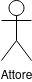
\includegraphics{../../img/Attore.png}
    \caption{Esempio di attore}
    \label{fig:attore}
\end{figure}

\begin{itemize}
    \item \textbf{Sistema}: Indica il contesto del sistema software, indicando funzionalità interne al contesto definito. \ref{fig:sistema} 
\end{itemize}

\begin{figure}[H]
    \centering
    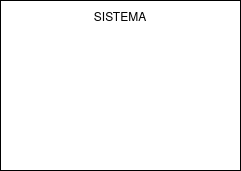
\includegraphics{../../img/sistema.png}
    \caption{Esempio di sistema}
    \label{fig:sistema}
\end{figure}

\begin{itemize}
    \item \textbf{Casi d’uso}: funzionalità offerte dal sistema che soddisfano le necessità di un Attore. Ogni caso d’uso descrive una sequenza specifica di interazioni tra gli attori e il sistema. \ref{fig:caso_uso}
\end{itemize}

\begin{figure}[H]
    \centering
    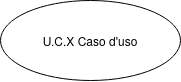
\includegraphics{../../img/CasoUso.png}
    \caption{Esempio di caso d'uso}
    \label{fig:caso_uso}
\end{figure}

\begin{itemize}
    \item \textbf{Sottocasi d’uso}: Scenari specifici che si verificano all'interno del caso d’uso principale. \ref{fig:sottocaso_uso}
\end{itemize}

\begin{figure}[H]
    \centering
    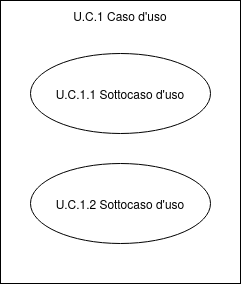
\includegraphics{../../img/Sottocasouso.png}
    \caption{Esempio di sottocaso d'uso}
    \label{fig:sottocaso_uso}
\end{figure}

\begin{itemize}
    \item \textbf{Relazioni tra Attori e Casi d’Uso}: 
    \begin{itemize}
        \item \textbf{Associazione}: Collegamento tra un attore e un caso d’uso, indicando che l’attore è coinvolto nel caso d’uso. \ref{fig:associazione}
    \end{itemize}
\end{itemize}

\begin{figure}[H]
    \centering
    \includegraphics{../../img/associazione.png}
    \caption{Esempio di associazione}
    \label{fig:associazione}
\end{figure}

\begin{itemize}
    \item \textbf{Relazioni tra Attori}:
    \begin{itemize}
        \item \textbf{Generalizzazione}: Un attore eredita le funzionalità di un altro attore. Una relazione padre figlio dove il figlio eredita almeno una funzionalità del padre. Utilizzata nel caso in cui due attori condividano funzionalità. \ref{fig:generalizzazione_casiuso}
    \end{itemize}
\end{itemize}

\begin{figure}[H]
    \centering
    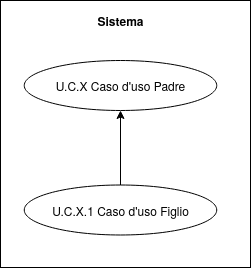
\includegraphics{../../img/Generalizzazione_casiuso.png}
    \caption{Esempio di Generalizzaione casi d'uso}
    \label{fig:generalizzazione_casiuso}
\end{figure}

\begin{itemize}
    \item \textbf{Relazioni tra Casi d’Uso}:
    \begin{itemize}
        \item \textbf{Inclusione}: Indica che un caso d’uso include un altro caso d’uso. Questo significa che durante l'esecuzione di un caso d'uso si eseguono anche i casi d'uso inclusi. Questo per evitare la ripetizione di funzionalità uguali in più casi d'uso. \ref{fig:inclusione}
    \end{itemize}
    

    \begin{figure}[H]
        \centering
        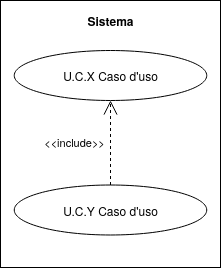
\includegraphics{../../img/include.png}
        \caption{Esempio di inclusione}
        \label{fig:inclusione}
    \end{figure}

    
    \begin{itemize}
        \item \textbf{Estensione}: Un caso d'uso esteso aggiunge funzionalità al caso d'uso principale, ma viene attivato solo in specifiche circostanze. Quando ciò accade, il flusso del caso d'uso principale si interrompe temporaneamente per consentire l'esecuzione del caso d'uso esteso. \ref{fig:estensione}
    \end{itemize}

    \begin{figure}[H]
        \centering
        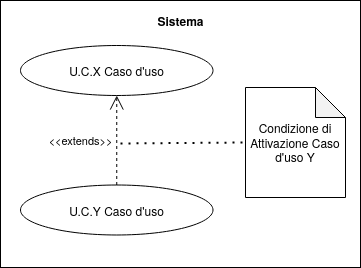
\includegraphics{../../img/estensione.png}
        \caption{Esempio di estensione}
        \label{fig:estensione}
    \end{figure}
    
    \begin{itemize}
        \item \textbf{Generalizzazione}: Un caso d'uso eredita le funzionalità di un altro caso d'uso. Una relazione padre figlio dove il figlio eredita almeno una funzionalità del padre. Utilizzata nel caso in cui due casi d'uso condividano funzionalità. \ref{fig:generalizzazione_attore}
    \end{itemize}

    \begin{figure}[H]
        \centering
        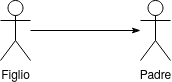
\includegraphics{../../img/Generalizzazione_Attori.png}
        \caption{Esempio di Generalizzaione attore}
        \label{fig:generalizzazione_attore}
    \end{figure}

\end{itemize}

\subsubsubsection{Requisiti}

I requisiti sono classificati in tre categorie principali:  
\begin{itemize}
    \item \textbf{Funzionali}: riguardano l'usabilità del prodotto finale;  
    \item \textbf{Di qualità}: includono gli strumenti e la documentazione da fornire;  
    \item \textbf{Di vincolo}: fanno riferimento alle tecnologie da utilizzare.
\end{itemize}
Ciascun requisito è indicato da:
\begin{itemize}
    \item \textbf{Codice Identificativo}: codice univoco che identifica il requisito;
    \item \textbf{Descrizione}: breve spiegazione del requisito;
    \item \textbf{Fonte}: origine del requisito (es. capitolato, interno, ecc..);
    \item \textbf{Priorità}: importanza del requisito rispetto agli altri;
\end{itemize} 

\subsubsubsection{Fonti dei requisiti}
I requisiti sono stati identificati a partire dalle seguenti fonti:
\begin{itemize}
    \item \textbf{Capitolato}: Requisiti individuati tramite analisi del capitolato;
    \item \textbf{interno}: requisiti individuati durante riunioni interne al gruppo di lavoro;
    \item \textbf{Esterno}: requisiti individuati durante incontri con il proponente;
    \item \href{https://code7crusaders.github.io/docs/RTB/documentazione_interna/glossario.html#piano-di-qualifica}{\textbf{Piano di Qualifica}\textsuperscript{G}}: Requisiti necessari per rispettare standard di qualità definiti nel documento \href{https://code7crusaders.github.io/docs/RTB/documentazione_interna/glossario.html#piano-di-qualifica}{Piano di Qualifica\textsuperscript{G}};
    \item \href{https://code7crusaders.github.io/docs/RTB/documentazione_interna/glossario.html#norme-di-progetto}{\textbf{Norme di Progetto}\textsuperscript{G}}: Requisiti necessari per rispettare le norme di progetto definite nel documento \href{https://code7crusaders.github.io/docs/RTB/documentazione_interna/glossario.html#norme-di-progetto}{Norme di Progetto\textsuperscript{G}};
\end{itemize}

\subsubsubsection{Codifica dei requisiti}
I requisiti sono codificati come segue: \textbf{R[Tipo][Importanza][Numero]}
\newline
Dove \textbf{Tipo} può essere:
\begin{itemize}
    \item \textbf{F (funzionale)}
    \item \textbf{Q (di qualità)}
    \item \textbf{V (di vincolo)}
\end{itemize}
\textbf{Importanza} può essere:
\begin{itemize}
    \item \textbf{O (obbligatorio)}
    \item \textbf{D (desiderabile)}
    \item \textbf{F (facoltativo )}
\end{itemize}
\textbf{Numero} è un numero identificativo univoco del requisito.
\subsubsubsection{Metriche}
\begin{table}[h!]
    \centering
    \renewcommand{\arraystretch}{1.5}
    \begin{tabular}{|>{\centering\arraybackslash}m{3cm}|>{\centering\arraybackslash}m{5cm}|}
        \hline
        \textbf{Metrica} & \textbf{Descrizione} \\
        \hline
        PRO & Percentuale Requisiti Obbligatori \\
        \hline
        PRD & Percentuale Requisiti Desiderabili \\
        \hline
        PRF & Percentuale Requisiti Facoltativi \\
        \hline
    \end{tabular}
    \caption{Percentuali requisiti}
    \label{tab:percentuali}
\end{table}

\subsubsection{Progettazione}
La fase di progettazione riveste un ruolo cruciale nel definire la struttura principale del progetto, basandosi sui requisiti individuati durante l'analisi e descritti nell’\href{https://code7crusaders.github.io/docs/RTB/documentazione_interna/glossario.html#analisi-dei-requisiti}{Analisi dei Requisiti\textsuperscript{G}}. Questa attività è affidata ai progettisti, i quali elaborano un piano dettagliato per implementare tutti i requisiti specificati.  
Per questa fase del ciclo di vita del software, il nostro gruppo si pone i seguenti obiettivi:
\begin{itemize}
    \item Trasformare i requisiti in specifiche tecniche dettagliate che coprano tutti gli aspetti del sistema.
    \item Garantire una struttura facilmente comprensibile per agevolare la manutenzione futura.
    \item Ottenere l’approvazione per il passaggio alla fase di sviluppo.
\end{itemize}
Il processo di progettazione si articola in tre livelli principali:
\begin{itemize}
    \item \textbf{Design dell’interfaccia}: questa fase si concentra su un livello di astrazione elevato rispetto al funzionamento interno del sistema. Durante la progettazione dell’interfaccia, l’attenzione è rivolta alle tecnologie da utilizzare nella fase di sviluppo del software, portando alla creazione di un \href{https://code7crusaders.github.io/docs/RTB/documentazione_interna/glossario.html#poc-proof-of-concept}{Proof of Concept\textsuperscript{G}}.
    \item \textbf{Progettazione architetturale}: si definisce la struttura generale del sistema a un alto livello, senza entrare nei dettagli interni dei componenti principali. In questa fase vengono anche definiti i test di integrazione.
    \item \textbf{Progettazione dettagliata}: si specificano gli elementi interni di ciascun componente principale, incluse le specifiche architetturali del prodotto. Si producono inoltre i diagrammi delle classi e si definiscono i test di unità per ogni componente. Questa fase culmina nella creazione della \href{https://code7crusaders.github.io/docs/RTB/documentazione_interna/glossario.html#pb-product-baseline}{Product Baseline\textsuperscript{G}}.
\end{itemize}

\subsubsection{Codifica}
Dopo la fase di progettazione, i membri del gruppo con il ruolo di Programmatori avviano la fase di codifica, 
implementando le specifiche dei requisiti e seguendo i documenti di progettazione.
L’obiettivo di questa fase è trasformare le idee in realtà, sviluppando il prodotto software desiderato tramite 
attività di programmazione. 
Le aspettative per la fase di codifica includono:
\begin{itemize}
    \item Completare lo sviluppo del prodotto finale garantendo la qualità e il rispetto delle richieste del committente;
    \item Assicurare che il codice prodotto sia chiaro e leggibile per facilitare eventuali modifiche future.
\end{itemize}
